\documentclass[12pt, letterpaper]{article}
\usepackage[utf8]{inputenc}
\usepackage{amsmath}
\usepackage{parskip}

\usepackage{graphicx}
\graphicspath{{../images/}}

\usepackage{hyperref}
\hypersetup{
    colorlinks=true,
    urlcolor=blue,
    linkcolor=blue,
    citecolor=blue,
    filecolor=blue,
}
\urlstyle{same}

\title{Notes to Preprocessing}
\author{}
\date{}


\begin{document}

\maketitle

\section{Feature Engineering}

Extending the original feature set with new informative covariates which are created from (combinations of) existing variables is a central aspect of every data analysis.
Besides many numeric features the Airbnb data contains \emph{images} as well as \emph{reviews} in raw text form.
These data types in particular require some preprocessing steps which will be the focus of this section.

In addition, some basic data cleaning steps were necessary.
These mostly consisted of converting data types, splitting text-based variables into more convenient numeric or boolean features and aggregating rare categories of categorical variables into one larger \emph{Other} group to stabilize estimation.
% COMMENT: nimmt vielleicht schon zu viel vor weg?

\subsection{Image Processing and Modeling}

Besides the metric and text-based features the Airbnb Data contains \emph{images} of the listed apartments as well as of the corresponding hosts.
This section describes how we used these images (while focusing on the apartment pictures) for the purpose of price prediction.

The main idea was to build a Convolutional Neural Network that predicts the price solely based on the image content itself and add these predictions as well as the number of available images for each listing to the main feature set.
Since there exist multiple images per apartment, the predictions were averaged afterwards within each group to obtain an output array of equal length to all remaining features.

\subsubsection{Webscraping}

In the first step, the raw image links provided by the data set had to converted to an image format that the neural network is able to work with.

Therefore we first used the \texttt{requests} library to get the \texttt{HTML} Source Code of each listing's website.
Next, the \texttt{beautifulsoup} library served as a convenient HTML parser to find and extract all embedded weblinks that lead to images located on the front page of the listings website.
With this strategy we could extract the first $5$ images for each apartment (if $5$ or more were available) that could be directly accessed from the front page source code.

Finally, we used the \texttt{requests} module again in combination with the \texttt{pillow} package to decode the source content of all image adresses into two dimensional images.


\subsubsection{Preprocessing}

Before feeding these two dimensional images into the model, we performed some further preprocessing steps.

One very common technique when dealing with images is \emph{Data Augmentation}.
In contrast to classification tasks however, where Data Augmentation is used to expand the training set and improve simultaneously generalization, this approach is not immediately transferable to a regression context since we have to guarantee that the label (i.e. the price) remains unchanged for each image transformation.
Thus, we decided against standard transformations such as rotating the images or manipulating the color composition.
% COMMENT: da wir das ja nicht weiter verfolgt haben: kürzer fassen? Ein Satz?

We \textbf{did} use image \emph{cropping}, however, which, in our opinion, is one of the few applicable augmentations in regression contexts.
After resizing all images to $256 \times 256$ pixels we randomly cropped a square area of $224 \times 224$ out of each image in the training set and cropped an equally sized area out of the image \textbf{center} in the validation set to avoid any randomness during inference.

At a final step all images were normalized, separately for each color channel.
In case of the pretrained model explained in the next section we used the same values for normilization that were used during training on the large \texttt{ImageNet} database.
The mean values and standard deviations for each color channel are provided in the \texttt{PyTorch} \href{https://pytorch.org/vision/stable/models.html}{documentation}.


\subsubsection{Modeling}

As mentioned above, we used a pretrained Convolutional Neural Network for modeling.
Ideally, due to learning from a large collection of labeled images in a supervised setting, this model is able to extract meaningful features from our own much smaller input data out of the box.
As usual in \emph{transfer learning} the weights of the pretrained model are frozen and the output layer is replaced by a trainable custom layer specific to our needs.
% COMMENT: Abkürzung für CNN einführen

One potential issue arises if the dataset used for pretraining differs from the new custom data:
If the pretrained network is very deep, the learned features before the final layer could be very specific to the Output Classes of \texttt{ImageNet} and not generalize well to our images.

There are multiple options to handle this scenario:
\begin{itemize}
    \item Out of the vast collection of freely available pretrained models, choose one that is comparably shallow.
          We chose \texttt{ResNet18} with roughly $11$ million parameters.
    \item Do not freeze the weights of the pretrained model completely, but rather fine tune them during training (i.e. modify \emph{all} weights by backpropagating through the entire network).
          We did not investigate this option further due to its high computational cost.
    \item Cut the pretrained model before the last layer with the hope that, at this point, very generic and widely applicable features of images are extracted.
          These features might in theory generalize better to our data.
          In practice, however, this option did not improve our results significantly.
\end{itemize}

It turned out that a \emph{single} custom layer, mapping from $512$ directly to a single neuron representing the scalar price prediction, was not expressive enough.
The performance improved by appending a (small) Fully Connected Network at the end instead containing three layers and \texttt{ReLU} activation functions.

To ensure that the chosen design is not majorly flawed, we constructed a separate much smaller Convolutional Neural Network with only a handful of Convolutional Blocks as a benchmark model.
Although the performance differences were not as large as desired, the pretrained \texttt{ResNet} indeed indicated more promising results.


\subsubsection{Results}

Using only the content of the available images, the pretrained \texttt{ResNet18} achieved a Mean Absolute Error of $579$ NOK (approx. $58$ Euros) on the Validation Set.
In comparison, the \emph{Null Model} of always predicting the mean price achieved an MAE of $630$ NOK without a log-transformation of the price and a MAE of $569$ NOK with a log-transformation.
Thus, the raw predictive power of the images alone was very small.

However, the \emph{correlation} of the CNN predictions with the true price was $0.41$.
This indicates some limitations of the correlation as useful metric on the one hand but at least positive tendencies of the CNN predictions on the other hand.
In fact, the network struggled the most with capturing the wide \emph{range} of prices and almost always predicted values close to the center of the (log) price distribution.

Although the general idea of categorizing images into price ranges based on image features sounds very appealing, taking a look at the actual input images reveals how challenging this task actually is.
Figure \ref{fig:cnn-examples} displays a random collection of input images.
Considering the difficulty of the task it is actually highly doubtful that humans could provide much more accurate predictions.

\section{Reviews}

In order to extract the most important information from the reviews, we have performed the following analyses.

First, we used the \texttt{langdetect} package to determine the language of each review.
With this information, we tried to get some insights about the internationality of the guests.
Since English and Norwegian are the most commonly used languages, we then created two so-called word clouds in this languages
to visualize the most frequently used words in the reviews and to give us a short overview of the given ratings.
To just have the important words in this representation, a list of given stop words are used to extract them.
What is most striking in the plots (s. Fig. \ref{fig:wordclouds}) is that in both predominantly positive words are printed. The largest printed and thus most frequently used words in English are \textit{apartement}, \textit{Oslo} and \textit{place} and
further \textit{clean}, \textit{comfortable}, \textit{helpful} and \textit{easy}. Also in the Norwegian plot there are mainly positive expressions like \textit{"anbefale"} (engl. recommend), \textit{"fin"} (engl. fine) and \textit{"flott leilighet"} (engl. great apartement).
% Wörter in Anführungsstriche oder kursiv?

% COMMENT: Example comment for Marei to show functionality :)
% insert Wordclouds english and norwegian side-by-side
\begin{figure}[t]
    \centering
    \begin{minipage}{6.7cm}
        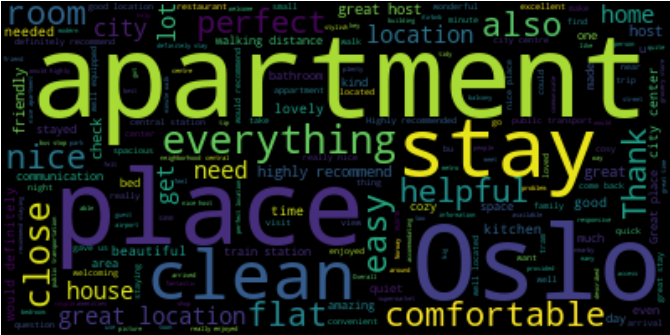
\includegraphics[width=\columnwidth]{wordcloud_eng.png}
    \end{minipage}
    \begin{minipage}{6.7cm}
        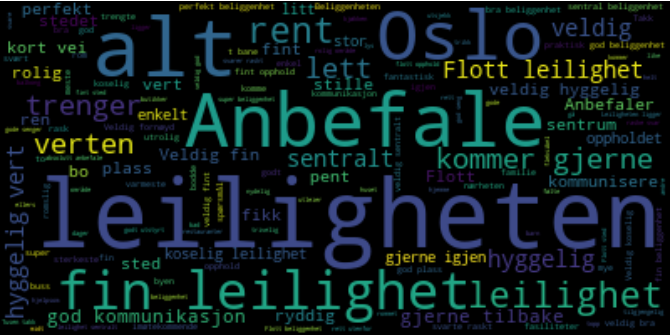
\includegraphics[width=\columnwidth]{wordcloud_nor.png}
    \end{minipage}
    \caption{Wordclouds in English and Norwegian}
    \label{fig:wordclouds}
\end{figure}

The results of the language detection are stored per \textit{listing\_id} in a new data frame called \textit{reviews\_features}.
This data frame contains the number of reviews per listing, the median length of a review, the number of different languages,
as well as a list of languages in which the reviews for that apartment were written. The percentages of Norwegian and English reviews are
also recorded for each listing id. Finally, this data frame was added to the \textit{listings} data frame on which feature selection
is performed later. (s. cite sentiment)

In addition, to obtain a more informed analysis of the reviews, we also performed a detailed sentiment analysis for each review. Sentiment analysis are used to detect the underlying emotion of a text. Therefore, it classifies the text as either positive or negative.
To do this, we used the \texttt{transformers} package, more specifically we used the \texttt{pipeline} function
with the \texttt{task} argument set to \textit{sentiment-analysis}, which is used for classifying sequences
according to positive or negative sentiments (s. documentation). The used model is DistlBERT,
a small, fast and light Transformer model, a distilled version of BERT algorithm, which achieves significantly faster results. (s. documentation transformers).
Finally, we used the sentiment analysis to determine the ratio of negative reviews to the total number of reviews per listings id, which is also added to the \textit{reviews\_feature} data frame.

%Sources:
%Analysis: https://towardsdatascience.com/a-beginners-guide-to-sentiment-analysis-in-python-95e354ea84f6
%Package: https://huggingface.co/transformers/v3.0.2/main_classes/pipelines.html
%Model: https://huggingface.co/transformers/v3.0.2/model_doc/distilbert.html


\section{Feature Selection}

Not all features out of the new combined and extended feature set are equally valuable to the model in terms of predictive power.
In fact, some of the features could not even be transformed to meaningful predictors such as multiple columns containing some kind of \texttt{id} information.
Others were completely redundant in presence of a combination of original and/or manually constructed features and were thus dropped from the feature set.

Before starting the modeling we intended to reduce the feature set even further to avoid strong correlations among the input predictors and possibly improve generalization performance to out-of-sample data.
Thus, we agreed on a two-step strategy.

First, we manually selected features based on three criteria:
%%%
\begin{enumerate}
    \item The variable in consideration and the apartment price must have some connection based on human intuition and background knowledge. For instance, we included variables containing information about the apartment's \emph{size} such as the number of \texttt{accomodates}, the number of \texttt{bathrooms} and the number of \texttt{bedrooms}.
    \item There has to exist some correlation with the price in a bivariate visualization, e.g. a \emph{barplot} in case of categorical predictors or a \emph{scatterplot} in case of numeric features.
    \item Since our dataset was comparably small with roughly $3000$ observations, we had to take care about missing values.
          Therefore, each variable whose missing values could not be imputed in a meaningful and uncontroversial manner was either selected or dropped based on the trade-off of the number of missing values reducing the size of the data set and its additional predictive value.
\end{enumerate}
%%%

Up to this point the feature selection process was solely based on bivariate relationships and self-chosen (arguably arbitrary) selection criteria.
There was a high chance of exluding important predictors that shine in combination with other variables rather than on their own.
% daher jetzt feature selection algorithms including
% -Schritt3: Manuelle Feature Selection bzw. inspiriert durch overall feature selection / Regression mit allen Features. Das Ergebnis hiervon ist dann listings_subset bzw. listings_extended
% -Schritt 5: Schritt 5 (optional): Automatisierte Feature Selection (zB durch RFE) bzw. Dimensionality Reduction (im Sinne von PCA) mittels eines Algorithmus

Therefore, in a second step we fitted an auxiliary Linear Regression Model with \emph{all} available features (except for the trivial ones such as the \verb|picture_url|) and analyzed the absolute magnitude of the coefficients to obtain the relevant coefficient here.
Since all variables are standardized, these magnitudes are within the same range and unit-independent and can thus be compared.

Of course, even this approach is not perfect, as several highly correlated characteristics that have a strong influence on price could lead to rather small estimated individual coefficients due to their joint predictive/explanatory power.
To circumvent this potential issue, we additionally used the \emph{algorithmic} feature selectors provided by the \texttt{scikit-learn} library, which (ideally) are able to separate the effects of highly correlated features and select only a small subset of them.

We decided to apply the following algorithms: \textit{RFE} (Recursive Feature Selection), \textit{SelectFromModel}, \textit{SelectKBest}, \textit{SequentialFeatureSelector} and \textit{VarianceThreshold}. The detailed results are given in the appendix.
Since \textit{RFE} showed the best performance and the selected subset of original features can be immediately interpreted as potentially the most important features, we then performed an even more detailed analysis using this feature selector.

% was sind unsere Ergebnisse der FSA zusammengefasst?
The overall results of these algorithms lead to the addition of the variable \texttt{property\_type}. But some of the observed correlations had to be taken with care. For example, the category \emph{houseboat} was assigned by far the largest coefficient of the variable \verb|property_type|.
However,  it turned out that this observation was the only houseboat included in the data set.
To avoid strong influences of these outliers, we combined all rare categories into one larger \texttt{Other} category and used the mean price of all observations included in this category.

The last step consists in preprocessing the data. For this purpose, we have implemented a \texttt{column\_transformer} function that includes both the One-Hot Encoding of the categorical variables and the standardization of the numerical variables and can be applied directly to an entire data set.


\section{Price Distribution}

One key aspect of exploratory data analysis is investigating the \emph{distribution} of the outcome variable.
In our case the price distribution is highly right-skewed with a few very expensive listings pulling the mean and median of the price distribution further away from each other.

Some statistical models such as \emph{Linear Regression} tend to perform better when the outcome distribution is symmetric and approximately normal, whereas some very flexible algorithms like \emph{Neural Networks} do not make any distributional assumptions and are capable of modeling any kind of distribution accurately.
Figure \ref{fig:price-distribution} illustrates an approximate normal distribution can be achieved with a simple logarithmic distribution.

Whereas \emph{all} of the classical models benefitted from the log-transformation resulting in lower error metrics, this was not the case for the Neural Network we used.

In fact, training turned out to be more challenging, since the \emph{magnitude} of the losses by comparing true and predicted price on the logarithmic scale was drastically reduced, leading to smaller gradients and thus smaller weight updates.
This issue could be mitigated to some extent with a larger learning rate.
However, in contrast to the untransformed version, the network still suffered from \emph{vanishing gradients} and \emph{loss plateaus}.



\newpage

\bibliography{bib}
\bibliographystyle{apalike}

\appendix

%%%
\begin{figure}[t]
    \centering
    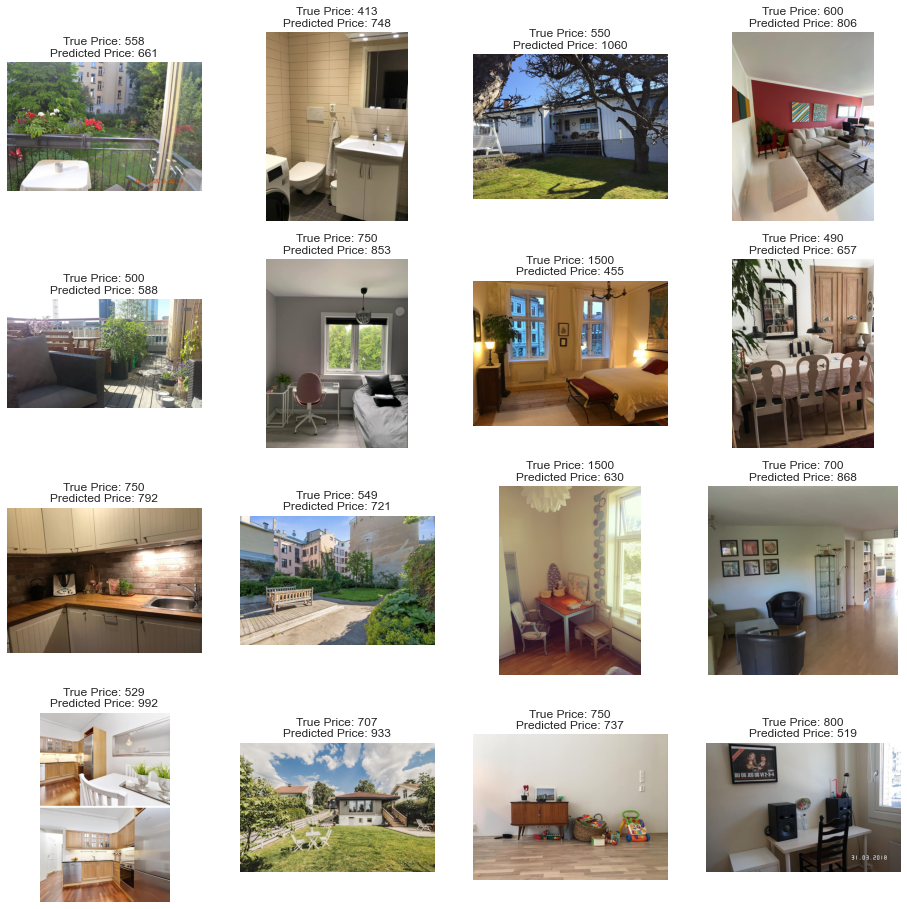
\includegraphics[width=\textwidth]{cnn_examples.png}
    \caption{Images from Airbnb Apartments with true and predicted Prices}
    \label{fig:cnn-examples}
\end{figure}
%%%

%%%
\begin{figure}[t]
    \centering
    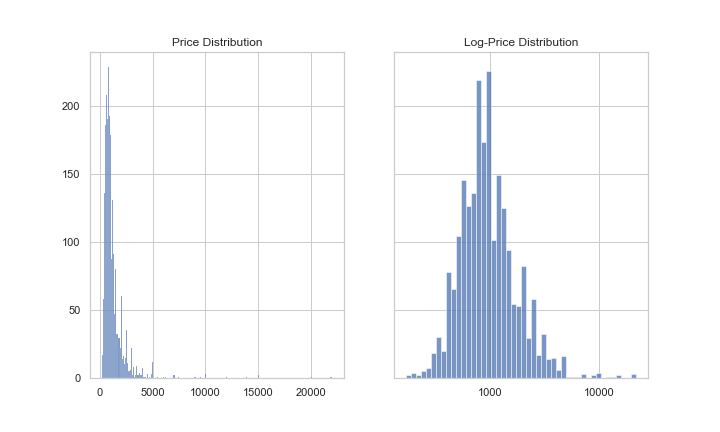
\includegraphics[width=0.8\textwidth]{price_distribution.png}
    \caption{Distribution of Apartment Prices on original and logarithmic Scale}
    \label{fig:price-distribution}
\end{figure}
%%%

\end{document}